\chapter{Figure Sample}

%IMPORTANT NOTE%
%Put the editable image source file (if this exists) in the Source folder!

                                                    % The fxnote is the reason that the caption
                                                    % is left aligned instead of centered.
                                                    % Furthermore, it does not show the fxnote in
\begin{figure}[H]                                   % a footnote.
  \centering                                        % It does however appear in list of corrections.
  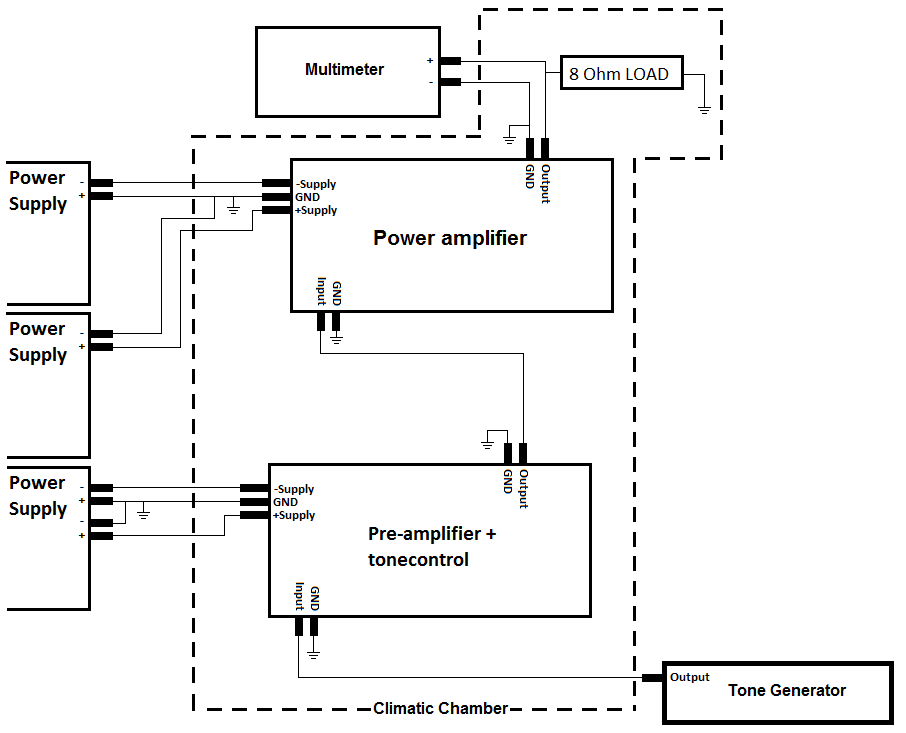
\includegraphics[scale=.3]{figures/filename}
  \caption{This image is clearly too small, remember to scale appropriately\fxnote{Remember source}}
  \label{FigureLABEL}     %<--give the figure a lable, so you can reference!
\end{figure}              %   For the label to work it must be under the caption.

%--------- NOTES ------------------------------------------------------
%Fxnotes wont compile properly inside the figure, only in the caption.
%File-type ([...]{figures/filename.jpg}) can be specified but isn't needed.
%
\Figref{FigureLABEL} $\leftarrow$ this is used in the beginning of a sentence, whereas \figref{HbridgeClokwise4Q} is used in the middle of a sentence\fxnote{This however does work in the footnote}.

%Do not use \vspace{length}, \hspace{length} or \noindent etc. unless exceedingly necessary - LaTeX is a markup language, let it do its job.
\vspace{.5cm}
\noindent
%--------- BIBLIOGRAPHY REF EKSAMPLE -----------------------------------
This reference only represents this line since it is before the punctuation mark\cite{YDing}. This next reference however represents the entire section. That is, all of the preceding sentences in the entire section. This is due to the fact that it is now after the punctuation mark in the end of the section (this is not used in the middle of a section!).\cite{YDing}
%>>>>>>>>>>>>>>>PLEASE ALSO READ THE NOTE IN bibliography/bibliography.bib<<<<<<<<<<<<<<<<<<

Here is a \st{good} messy way to make two images appear on the side of each other. Also, if you modified an image, this is how you properly refer to its original source:

  \begin{minipage}{\linewidth}
  	\begin{minipage}{0.45\linewidth}
  		\begin{figure}[H]
  			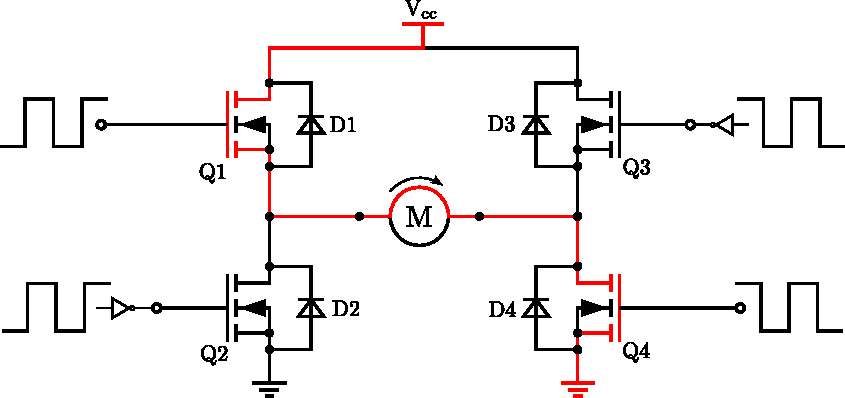
\includegraphics[scale=.53]{figures/HbridgeClockwise4Q.pdf}
  			\centering
  			\vspace{-.4cm}
  			\captionsetup{justification=centering}
  			\captionof{figure}{Clockwise 4Q operation.\\ \emph{Edited from image by Biezl}.\cite{Biezl}}
  			\label{HbridgeClokwise4Q}
  		\end{figure}\vspace{-5mm}
  	\end{minipage}
  	\hspace{0.03\linewidth}
  	\begin{minipage}{0.45\linewidth}
  		\begin{figure}[H]
  			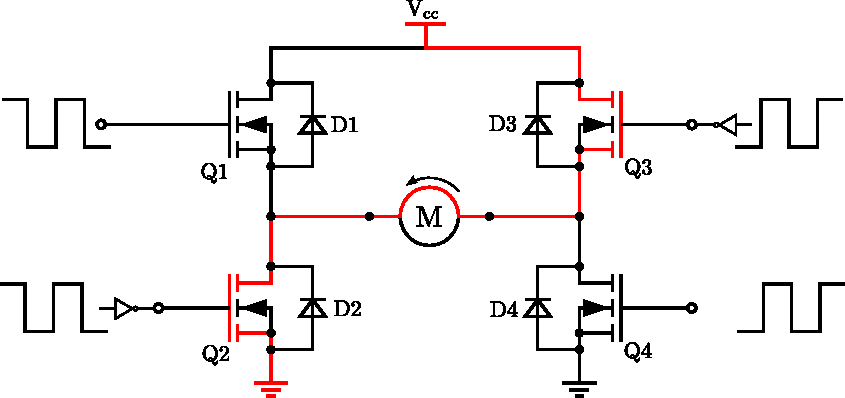
\includegraphics[scale=.53]{figures/HbridgeCounterClockwise4Q.pdf}
  			\centering
  			\vspace{-.4cm}
  			\captionsetup{justification=centering}
  			\captionof{figure}{Counterclockwise 4Q operation.\\ \emph{Edited from image by Biezl}.\cite{Biezl}}
  			\label{HbridgeCounterClokwise4Q}
  		\end{figure}\vspace{-5mm}
  	\end{minipage}
  \end{minipage}

\pagebreak